\subsection{Relation to Bell Inequalities}
\label{subsec:relation-to-bell-inequalities}

Bell's theorem~\cite{Bell1964} rules out any ontological completion of
quantum mechanics based on factorizable hidden-variable models.
Cosmochrony fully accepts Bell's theorem and identifies the ontological
assumption that fails: the factorization hypothesis $P(a,b|x,y,\lambda) = P(a|x,\lambda)\,P(b|y,\lambda)$.

Because the projection~$\Pi$ is generically non-injective, admissible
projected states are not associated with independent ontic pre-images for their subsystems.
The factorization hypothesis is not merely violated but \emph{ill-defined}
within the space of admissible projected descriptions.

Bell-type violations arise in an intermediate regime of projective
compression: the effective description is sufficiently coarse-grained to
permit subsystem separation, yet retains enough global relational structure to prevent factorization.
In the limit of extreme coarse-graining, projected descriptions become effectively classical.

\begin{figure}[t]
  \centering
  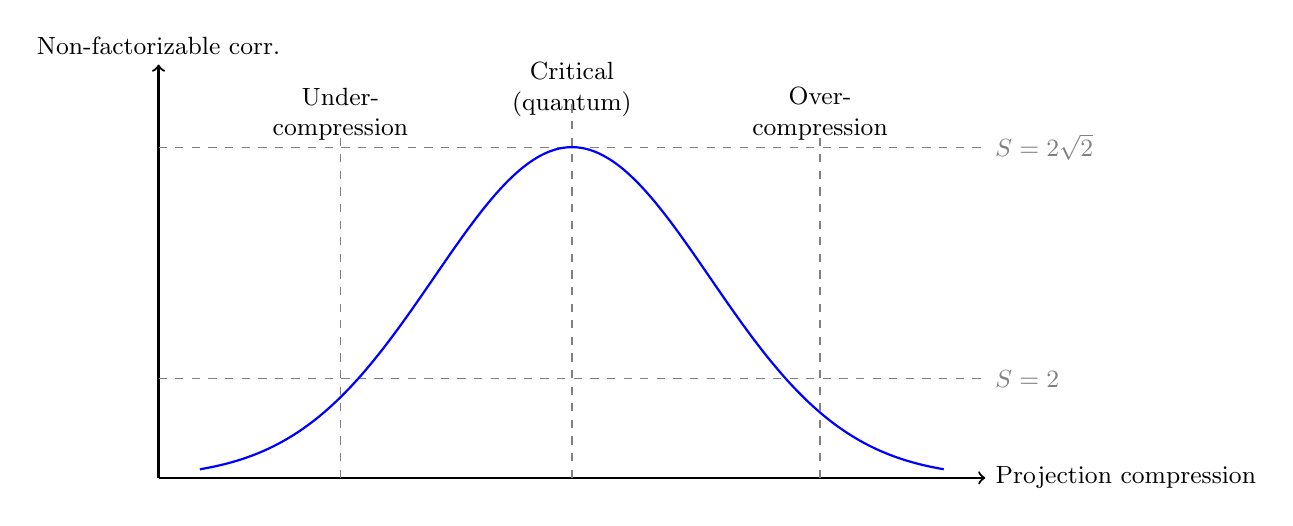
\begin{tikzpicture}[
    scale=1.05,
    axis/.style={->, thick},
    curve/.style={thick, smooth, blue},
    dashedline/.style={dashed, gray},
    label/.style={font=\small}
  ]
    \draw[axis] (0,0) -- (10,0)
      node[right,label] {Projection compression};
    \draw[axis] (0,0) -- (0,5)
      node[above,label] {Non-factorizable corr.};
    \draw[dashedline] (0,1.2) -- (10,1.2)
      node[right,label] {$S=2$};
    \draw[dashedline] (0,4) -- (10,4)
      node[right,label] {$S=2\sqrt{2}$};
    \draw[curve]
      plot[domain=0.5:9.5,samples=200]
      (\x,{4*exp(-0.18*(\x-5)^2)});
    \node[label, align=center] at (2.2,4.4)
      {Under-\\compression};
    \node[label, align=center] at (5,4.7)
      {Critical\\(quantum)};
    \node[label, align=center] at (8,4.4)
      {Over-\\compression};
    \draw[dashedline] (2.2,0) -- (2.2,4.2);
    \draw[dashedline] (5,0) -- (5,4.6);
    \draw[dashedline] (8,0) -- (8,4.2);
  \end{tikzpicture}
  \caption{Bell inequality violations as a function of the
    compression induced by~$\Pi$.
    Non-factorizable correlations emerge in an intermediate regime.}
  \label{fig:bell-compression-regime}
\end{figure}

No hidden variables and no superluminal influence are introduced.
Quantum nonlocality is ontological rather than dynamical: the failure of
Bell-type factorizability arises from the structure of admissible projected descriptions, not from nonlocal interaction.
